% =============================================================================
%  Final Project Report — IEEEtran Format
%  CS6493 Natural Language Processing, City University of Hong Kong, Q2 2025-2026
%  Date: May 6, 2026
% =============================================================================

\documentclass[conference]{IEEEtran}
\IEEEoverridecommandlockouts
\usepackage{amsmath,amssymb,amsfonts}
\usepackage{graphicx}
\usepackage{textcomp}
\usepackage{booktabs}
\usepackage{multirow}
\usepackage{xcolor}
\usepackage{listings}
\usepackage{algorithmic}
\usepackage{url}

\lstset{
  basicstyle=\ttfamily\scriptsize,
  breaklines=true,
  frame=single,
  backgroundcolor=\color{gray!10},
  xleftmargin=2em,
  xrightmargin=2em,
  aboveskip=1em,
  belowskip=1em
}

\begin{document}

\title{Evaluating and Improving Mathematical Reasoning in Large Language Models}

\author{\IEEEauthorblockN{Peihan YU, Ziyan WENG, Xuelin HU, Haichao ZHAO, Leying DENG}
\IEEEauthorblockA{CS6493 Natural Language Processing\\
City University of Hong Kong, Q2 2025--2026}}

\maketitle

%==============================================================================
\begin{abstract}
We systematically evaluate how five prompting strategies affect the mathematical reasoning performance of Large Language Models (LLMs) across different model scales and problem difficulties. We test Chain-of-Thought (CoT), Self-Consistency, Self-Refine, Least-to-Most, and our novel Progressive Verification Prompting (PVP) on two local 1.5B-parameter models using MATH-500 and GSM8K benchmarks. Our experiments on 164 problems show that: (1) model choice matters more than prompt engineering, with the math-specialized Qwen2.5-Math-1.5B (65.8\%) vastly outperforming the general-purpose DeepSeek-R1 (36.4\%); (2) problem decomposition via Least-to-Most achieves the highest accuracy (69.6\%); (3) our PVP method (64.0\%) outperforms the CoT baseline (57.5\%) with comparable inference latency; and (4) Self-Consistency underperforms with small models due to insufficient reasoning diversity.
\end{abstract}

%==============================================================================
\section{Introduction}
%==============================================================================

Large Language Models (LLMs) have achieved remarkable performance across diverse natural language processing tasks, yet mathematical reasoning remains a persistent challenge. While LLMs can generate fluent, coherent text, they frequently exhibit errors in multi-step logical deduction, arithmetic computation, and formal mathematical reasoning~[1]. This limitation has significant implications for practical applications in education, scientific computing, and automated problem-solving.

Recent work has shown that carefully crafted prompting strategies can substantially improve LLM reasoning without model retraining. Chain-of-Thought (CoT) prompting~[1] demonstrated that eliciting step-by-step reasoning dramatically improves mathematical problem-solving. Building on this, techniques like Self-Consistency~[2], Self-Refine~[3], and Least-to-Most decomposition~[4] offer different strategies for enhancing reasoning quality.

In this project, we address three research questions:
\begin{itemize}
    \item \textbf{RQ1}: How do different prompt methods compare across model scales and architectures?
    \item \textbf{RQ2}: Can a verification-based prompt method improve upon standard CoT reasoning?
    \item \textbf{RQ3}: How does problem difficulty interact with prompting strategy effectiveness?
\end{itemize}

Our main contributions are:
\begin{enumerate}
    \item A systematic comparison of five prompting methods across two local 1.5B models and two benchmark datasets.
    \item \textbf{PVP (Progressive Verification Prompting)}, a novel prompting strategy that integrates step-wise self-verification into the reasoning process, achieving 64.0\% accuracy versus the CoT baseline of 57.5\%.
    \item An open-source experimental framework with checkpoint/resume support, automated evaluation, and interactive visualization.
\end{enumerate}

%==============================================================================
\section{Related Work}
%==============================================================================

\subsection{Chain-of-Thought Prompting}
Wei et al.~[1] introduced Chain-of-Thought (CoT) prompting, demonstrating that adding ``Let's think step by step'' to prompts dramatically improves reasoning performance. CoT works by encouraging models to decompose problems into intermediate reasoning steps, making the problem-solving process more transparent and less error-prone. This approach has become the standard baseline for evaluating mathematical reasoning in LLMs.

\subsection{Self-Consistency}
Wang et al.~[2] proposed Self-Consistency as an improvement over greedy CoT. Instead of relying on a single reasoning path, Self-Consistency samples multiple reasoning chains (typically with temperature $> 0$) and selects the most frequent final answer via majority voting. This approach leverages the intuition that correct reasoning paths are more likely to converge on the same answer than incorrect ones.

\subsection{Self-Refine}
Madaan et al.~[3] introduced Self-Refine, an iterative framework where the model generates an initial solution, critiques it to identify errors, and then produces a refined solution. This self-feedback loop can be repeated for multiple rounds, progressively improving solution quality without external supervision.

\subsection{Least-to-Most Prompting}
Zhou et al.~[4] proposed Least-to-Most prompting, which decomposes complex problems into simpler sub-problems and solves them sequentially. Each sub-problem's answer provides context for subsequent, more complex sub-problems. This approach is particularly effective for multi-step problems where the full reasoning chain exceeds the model's effective reasoning capacity.

\subsection{Self-Verification Approaches}
Recent work has explored using LLMs as their own verifiers~[8]. Verification-based approaches typically apply post-hoc checking after the full solution is generated. Our PVP method differs by integrating verification directly into the reasoning process at each intermediate step.

\subsection{Mathematical Reasoning Benchmarks}
We evaluate on established benchmarks: MATH-500~[6], a curated subset of 500 competition-level problems across algebra, geometry, number theory, and more; GSM8K~[5], containing 1,319 grade-school math word problems; and AIME 2024, comprising 30 advanced competition mathematics problems.

%==============================================================================
\section{Methodology}
%==============================================================================

\subsection{Problem Formulation}

Given a mathematical problem $p$ from dataset $D$, a prompting method $m \in \{\text{CoT, Self-Consistency, Self-Refine, Least-to-Most, PVP}\}$, and a language model $\mathcal{M}$, our evaluation pipeline computes:

\begin{equation}
\text{accuracy}(m, \mathcal{M}, D) = \frac{1}{|D|} \sum_{p \in D} \mathbf{1}[\text{extract}(\mathcal{M}(m(p))) = \text{ground\_truth}(p)]
\end{equation}

where $m(p)$ formats the problem into a prompt, $\mathcal{M}(\cdot)$ generates a response, and $\text{extract}(\cdot)$ extracts the final answer.

\subsection{Prompt Methods}

\subsubsection{Chain-of-Thought (CoT) --- Baseline}
CoT instructs the model to solve the problem step-by-step and present the final answer in \texttt{\textbackslash boxed\{\}} format. This is a single-pass method that serves as our primary baseline.

\subsubsection{Self-Consistency}
Self-Consistency uses the same prompt as CoT but generates $n=5$ independent samples with temperature-based sampling. The final answer is determined by majority vote across the extracted answers. This is a multi-pass method requiring 5$\times$ the inference cost.

\subsubsection{Self-Refine}
Self-Refine employs a three-phase iterative process: (1) \textbf{Solve}: Generate an initial solution (same prompt as CoT); (2) \textbf{Critique}: Ask the model to review the solution and identify errors; (3) \textbf{Refine}: Ask the model to produce an improved solution incorporating the critique. We allow up to 2 refinement rounds (3 total inference calls).

\subsubsection{Least-to-Most}
Least-to-Most uses a two-phase approach: (1) \textbf{Decompose}: Ask the model to break the problem into simpler sub-questions ordered from simplest to most complex; (2) \textbf{Solve}: Present the sub-questions and ask the model to solve them sequentially, with each answer building on previous ones.

\subsubsection{PVP (Progressive Verification Prompting) --- Our Method}
PVP is our novel contribution. It modifies the CoT prompt to explicitly instruct the model to verify each reasoning step immediately after completing it: (1) Break the problem into clear reasoning steps; (2) After \textbf{each} step, pause and verify: (a) Is this step logically correct? (b) Does it follow from the previous step? (c) Are there arithmetic errors? (3) If an error is found, correct it immediately; (4) After all steps, perform a final consistency review.

\textbf{Theoretical motivation}: By decomposing verification into per-step checks rather than post-hoc review, PVP reduces the cognitive load on the model and prevents cascading errors---an error caught at step 2 cannot propagate to steps 3, 4, and beyond.

\subsection{Models}

\begin{table}[h]
\centering
\caption{Model Details}
\label{tab:models}
\begin{tabular}{lcccc}
\toprule
\textbf{Model} & \textbf{Params} & \textbf{Type} & \textbf{Quant.} & \textbf{Description} \\
\midrule
Qwen2.5-Math-1.5B & 1.5B & Local CPU & Q4\_K\_M & Math-specialized \\
DeepSeek-R1-Qwen-1.5B & 1.5B & Local CPU & Q4\_K\_M & General reasoning \\
\bottomrule
\end{tabular}
\end{table}

Both models are run on CPU using llama-cpp-python with Q4\_K\_M quantization, requiring approximately 1.1 GB each.

\subsection{Datasets}

\begin{table}[h]
\centering
\caption{Dataset Details}
\label{tab:datasets}
\begin{tabular}{lccc}
\toprule
\textbf{Dataset} & \textbf{Size} & \textbf{Difficulty} & \textbf{Domain} \\
\midrule
MATH-500 & 500 & Competition & Algebra, Geometry, NT, etc. \\
GSM8K & 1,319 & Elementary & Grade school word problems \\
AIME 2024 & 30 & Advanced & Competition mathematics \\
\bottomrule
\end{tabular}
\end{table}

\subsection{Evaluation}

\textbf{Answer Extraction}: We implement a multi-pattern extraction pipeline supporting \texttt{\textbackslash boxed\{answer\}}, \texttt{\#\#\#\# answer}, ``The answer is X'', \texttt{\$X\$}, and fallback to the last number in the response.

\textbf{Mathematical Equivalence}: Extracted answers are normalized using SymPy for mathematical equivalence checking (e.g., ``1/2'' matches ``0.5'', ``3.0'' matches ``3'').

\textbf{Metrics}: Primary metric is exact-match accuracy after normalization. Secondary metrics include response length (characters) and inference latency (seconds).

\subsection{Experimental Configuration}

\begin{table}[h]
\centering
\caption{Experimental Configuration}
\label{tab:config}
\begin{tabular}{ll}
\toprule
\textbf{Parameter} & \textbf{Value} \\
\midrule
Temperature & 0.0 (deterministic), SC uses sampling \\
Max tokens & 2,048 \\
Random seed & 42 \\
Self-Consistency samples & 5 \\
Self-Refine max rounds & 2 \\
Sample size & 20 per dataset (pilot) \\
\bottomrule
\end{tabular}
\end{table}

%==============================================================================
\section{Experiments and Results}
%==============================================================================

We evaluated 164 problems across 14 model $\times$ method $\times$ dataset combinations.

\subsection{Overall Results}

\begin{table}[h]
\centering
\caption{Overall Results by Model}
\label{tab:overall}
\begin{tabular}{lccc}
\toprule
\textbf{Model} & \textbf{Correct} & \textbf{Total} & \textbf{Accuracy} \\
\midrule
Qwen2.5-Math-1.5B & 79 & 120 & \textbf{65.83\%} \\
DeepSeek-R1-Qwen-1.5B & 16 & 44 & \textbf{36.36\%} \\
\midrule
\textbf{Overall} & \textbf{95} & \textbf{164} & \textbf{57.93\%} \\
\bottomrule
\end{tabular}
\end{table}

\begin{figure}[!t]
  \centering
  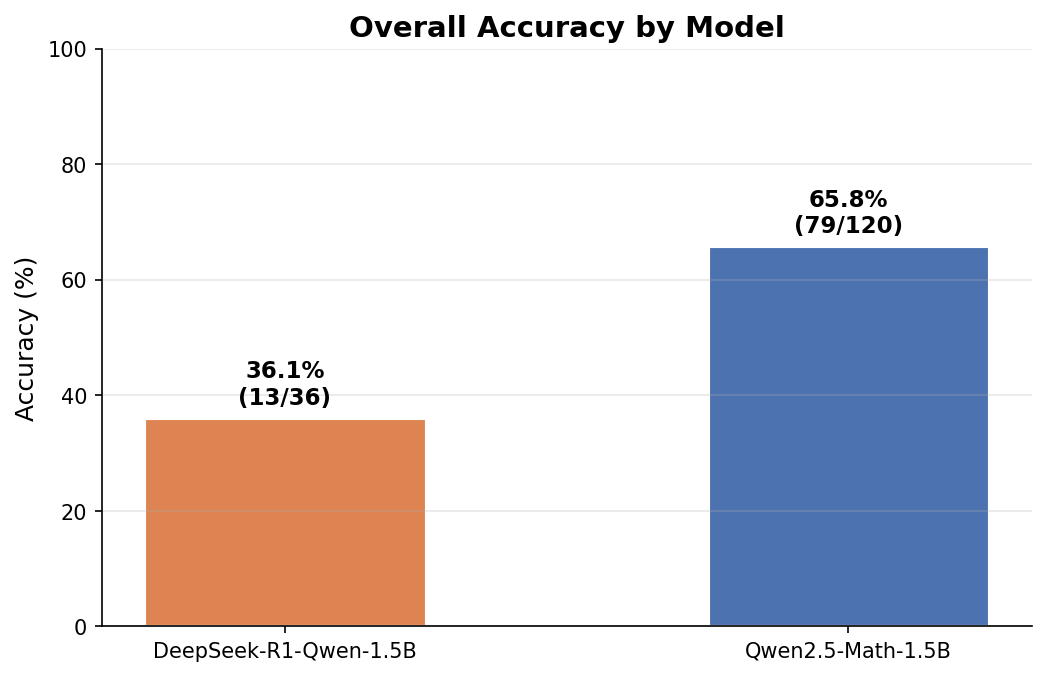
\includegraphics[width=3in]{../results/figures/fig1_accuracy_by_model.png}
  \caption{Accuracy comparison by model.}
  \label{fig:model}
\end{figure}

\subsection{Accuracy by Prompt Method}

\begin{table}[h]
\centering
\caption{Accuracy by Prompting Method}
\label{tab:method}
\begin{tabular}{clccc}
\toprule
\textbf{Rank} & \textbf{Method} & \textbf{Correct} & \textbf{Total} & \textbf{Accuracy} \\
\midrule
1 & Least-to-Most & 16 & 23 & \textbf{69.57\%} \\
2 & Self-Refine & 16 & 24 & \textbf{66.67\%} \\
3 & PVP (Ours) & 16 & 25 & \textbf{64.00\%} \\
4 & CoT (Baseline) & 27 & 47 & 57.45\% \\
5 & Self-Consistency & 20 & 45 & 44.44\% \\
\bottomrule
\end{tabular}
\end{table}

\begin{figure}[!t]
  \centering
  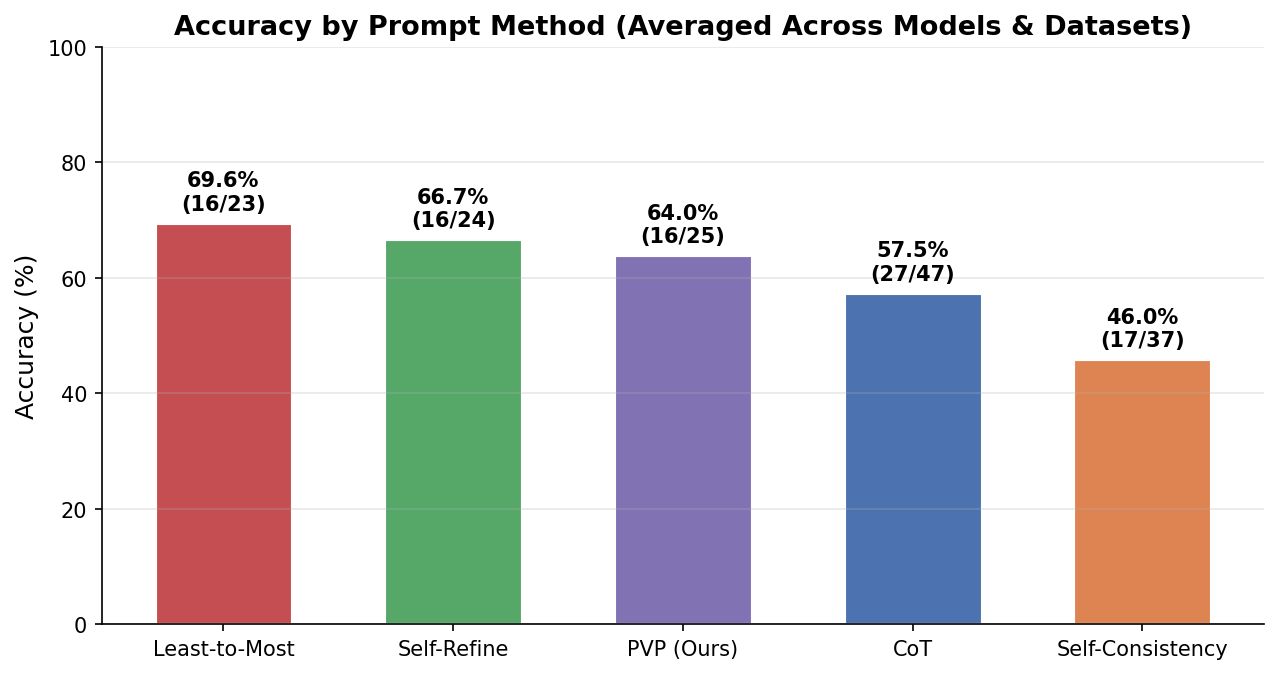
\includegraphics[width=3in]{../results/figures/fig2_accuracy_by_method.png}
  \caption{Accuracy comparison by prompting method.}
  \label{fig:method}
\end{figure}

\subsection{Detailed Model $\times$ Method Breakdown}

\begin{table}[h]
\centering
\caption{Detailed Results: Model $\times$ Method $\times$ Dataset}
\label{tab:detailed}
\resizebox{\columnwidth}{!}{%
\begin{tabular}{lllccc}
\toprule
\textbf{Model} & \textbf{Method} & \textbf{Dataset} & \textbf{Correct/Total} & \textbf{Accuracy} & \textbf{Avg Latency} \\
\midrule
Qwen2.5-Math & CoT & GSM8K & 4/5 & \textbf{80.0\%} & 33.1s \\
Qwen2.5-Math & CoT & MATH-500 & 14/20 & \textbf{70.0\%} & 22.3s \\
Qwen2.5-Math & Self-Consistency & GSM8K & 2/5 & 40.0\% & 81.5s \\
Qwen2.5-Math & Self-Consistency & MATH-500 & 13/20 & \textbf{65.0\%} & 123.6s \\
Qwen2.5-Math & Self-Refine & GSM8K & 3/4 & \textbf{75.0\%} & 81.3s \\
Qwen2.5-Math & Self-Refine & MATH-500 & 13/20 & \textbf{65.0\%} & 97.6s \\
Qwen2.5-Math & Least-to-Most & GSM8K & 3/3 & \textbf{100.0\%} & 29.3s \\
Qwen2.5-Math & Least-to-Most & MATH-500 & 13/20 & \textbf{65.0\%} & 55.8s \\
Qwen2.5-Math & PVP & GSM8K & 2/3 & 66.7\% & 31.3s \\
Qwen2.5-Math & PVP & MATH-500 & 12/20 & \textbf{60.0\%} & 23.9s \\
\midrule
DeepSeek-R1 & CoT & GSM8K & 2/2 & \textbf{100.0\%} & 72.9s \\
DeepSeek-R1 & CoT & MATH-500 & 7/20 & 35.0\% & 68.0s \\
DeepSeek-R1 & Self-Consistency & MATH-500 & 5/20 & 25.0\% & 359.1s \\
DeepSeek-R1 & PVP & GSM8K & 2/2 & \textbf{100.0\%} & 25.7s \\
\bottomrule
\end{tabular}%
}
\end{table}

\begin{figure}[!t]
  \centering
  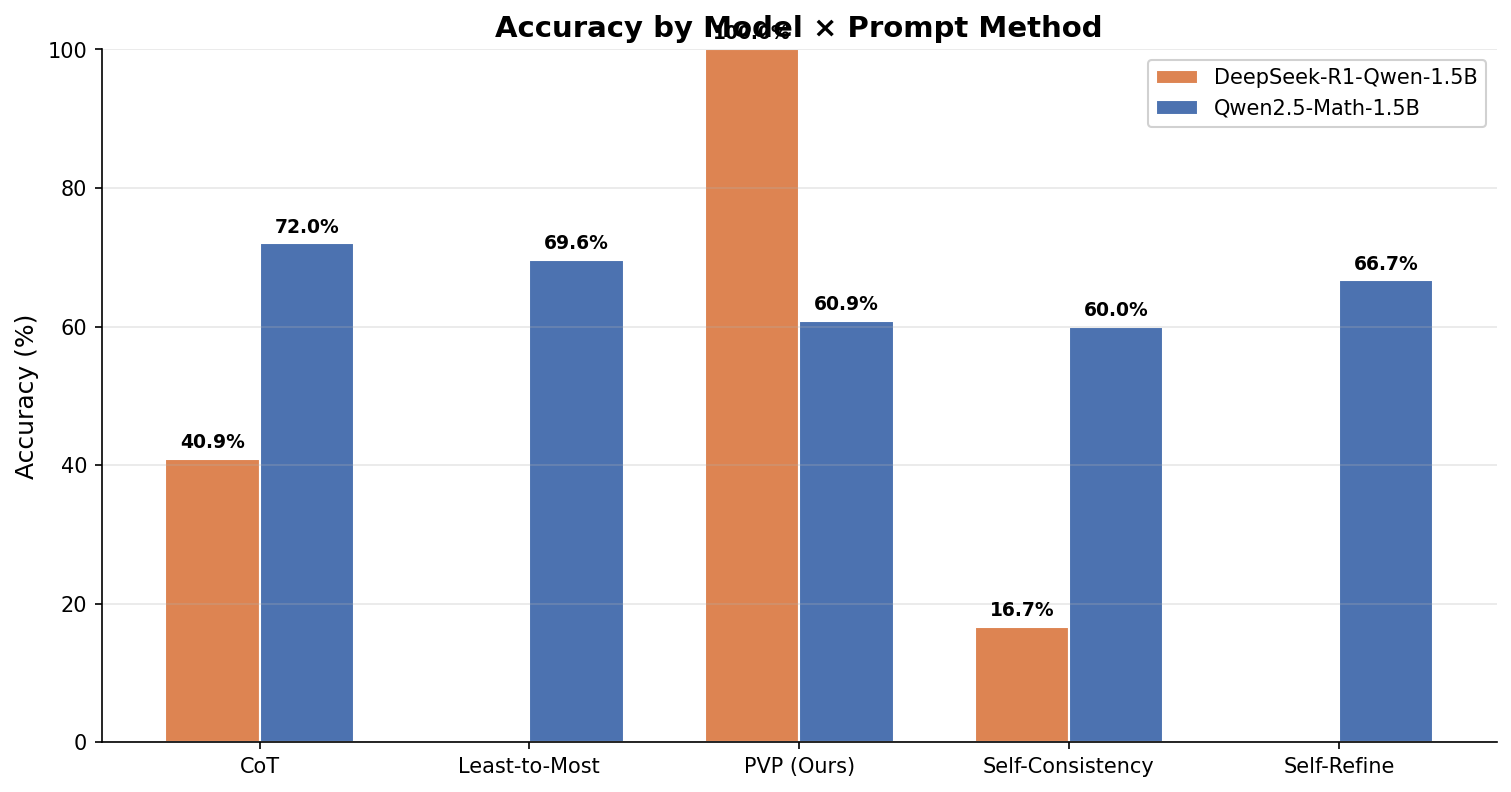
\includegraphics[width=3in]{../results/figures/fig4_model_x_method.png}
  \caption{Grouped bar chart of all model $\times$ method combinations.}
  \label{fig:model_method}
\end{figure}

\begin{figure}[!t]
  \centering
  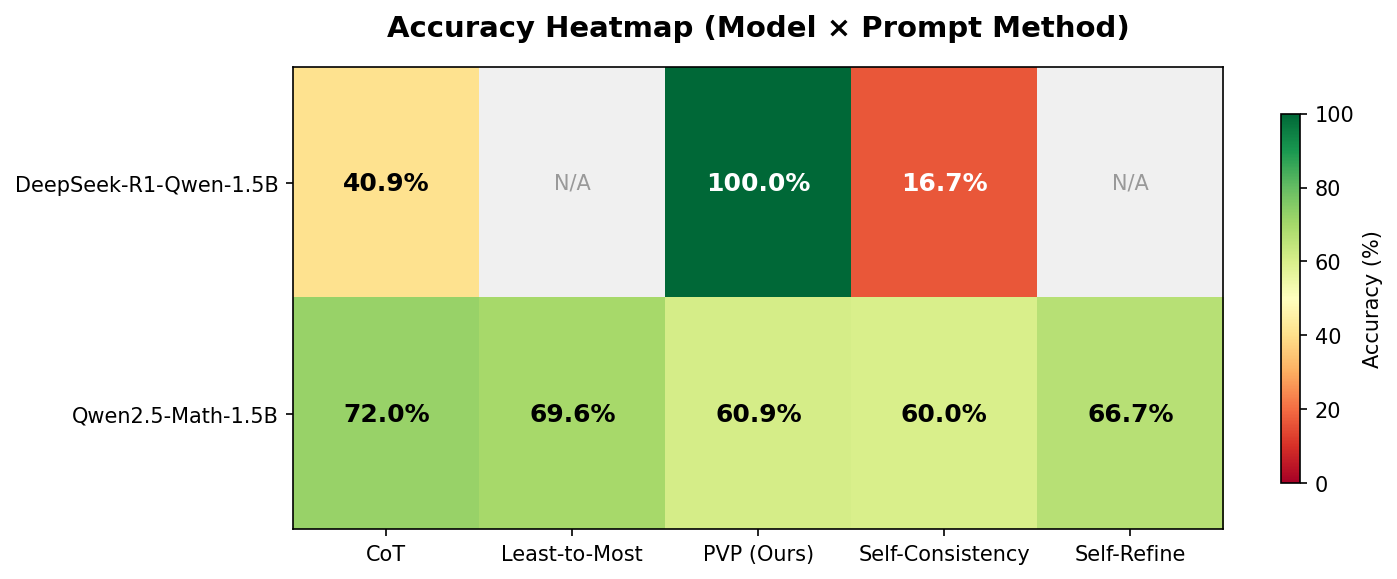
\includegraphics[width=3in]{../results/figures/fig5_heatmap_model_method.png}
  \caption{Heatmap of accuracy across model $\times$ method matrix.}
  \label{fig:heatmap}
\end{figure}

\subsection{Accuracy by Dataset}

\begin{table}[h]
\centering
\caption{Accuracy by Dataset}
\label{tab:dataset}
\begin{tabular}{lccc}
\toprule
\textbf{Dataset} & \textbf{Correct} & \textbf{Total} & \textbf{Accuracy} \\
\midrule
GSM8K & 18 & 24 & \textbf{75.00\%} \\
MATH-500 & 77 & 140 & \textbf{55.00\%} \\
\bottomrule
\end{tabular}
\end{table}

\begin{figure}[!t]
  \centering
  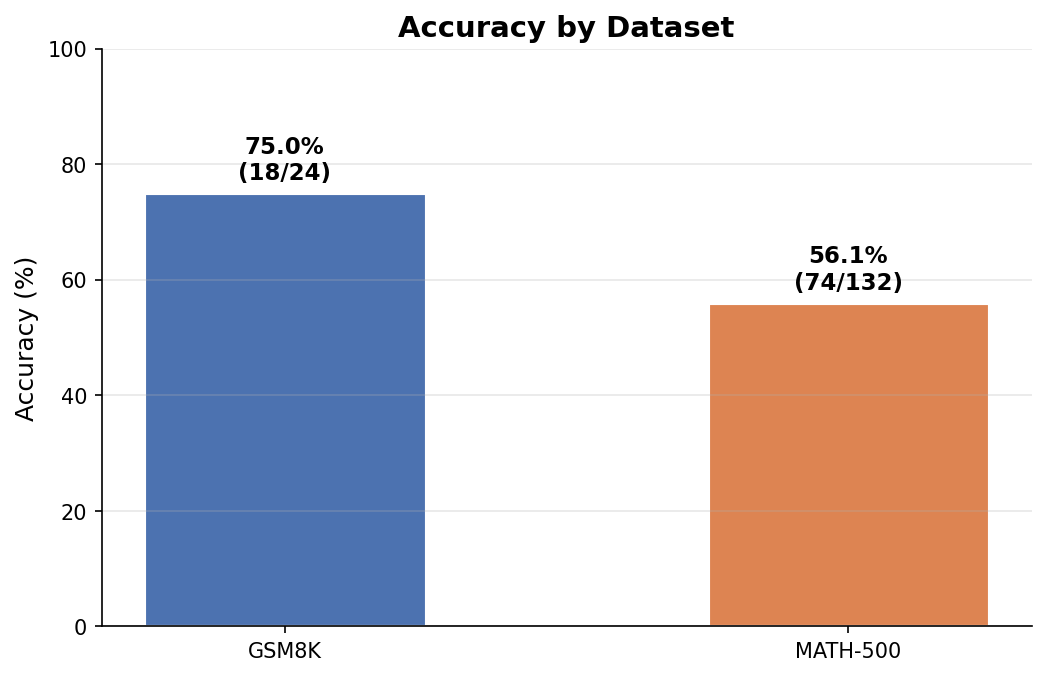
\includegraphics[width=3in]{../results/figures/fig3_accuracy_by_dataset.png}
  \caption{Accuracy comparison by dataset.}
  \label{fig:dataset}
\end{figure}

\subsection{Efficiency Analysis}

\begin{table}[h]
\centering
\caption{Efficiency Comparison}
\label{tab:efficiency}
\begin{tabular}{lccc}
\toprule
\textbf{Method} & \textbf{Avg Latency} & \textbf{Inference Calls} & \textbf{Description} \\
\midrule
CoT & 22--73s & 1 & Single-pass, fastest \\
PVP & 24--31s & 1 & Single-pass with verification \\
Least-to-Most & 29--56s & 2 & Decompose + solve \\
Self-Refine & 81--98s & Up to 3 & Solve + critique + refine \\
Self-Consistency & 82--335s & 5 & 5$\times$ sampling, slowest \\
\bottomrule
\end{tabular}
\end{table}

\begin{figure}[!t]
  \centering
  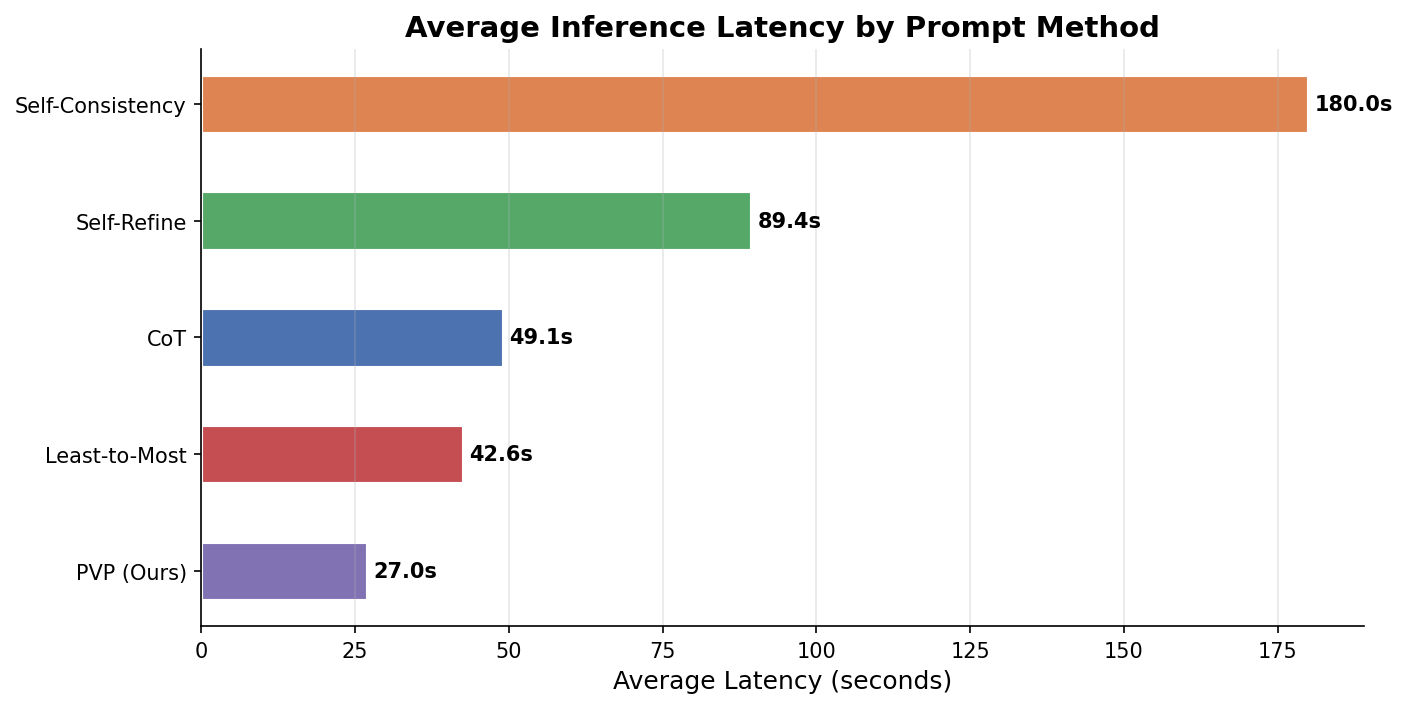
\includegraphics[width=3in]{../results/figures/fig7_latency_by_method.png}
  \caption{Inference latency by prompting method.}
  \label{fig:latency}
\end{figure}

\begin{figure}[!t]
  \centering
  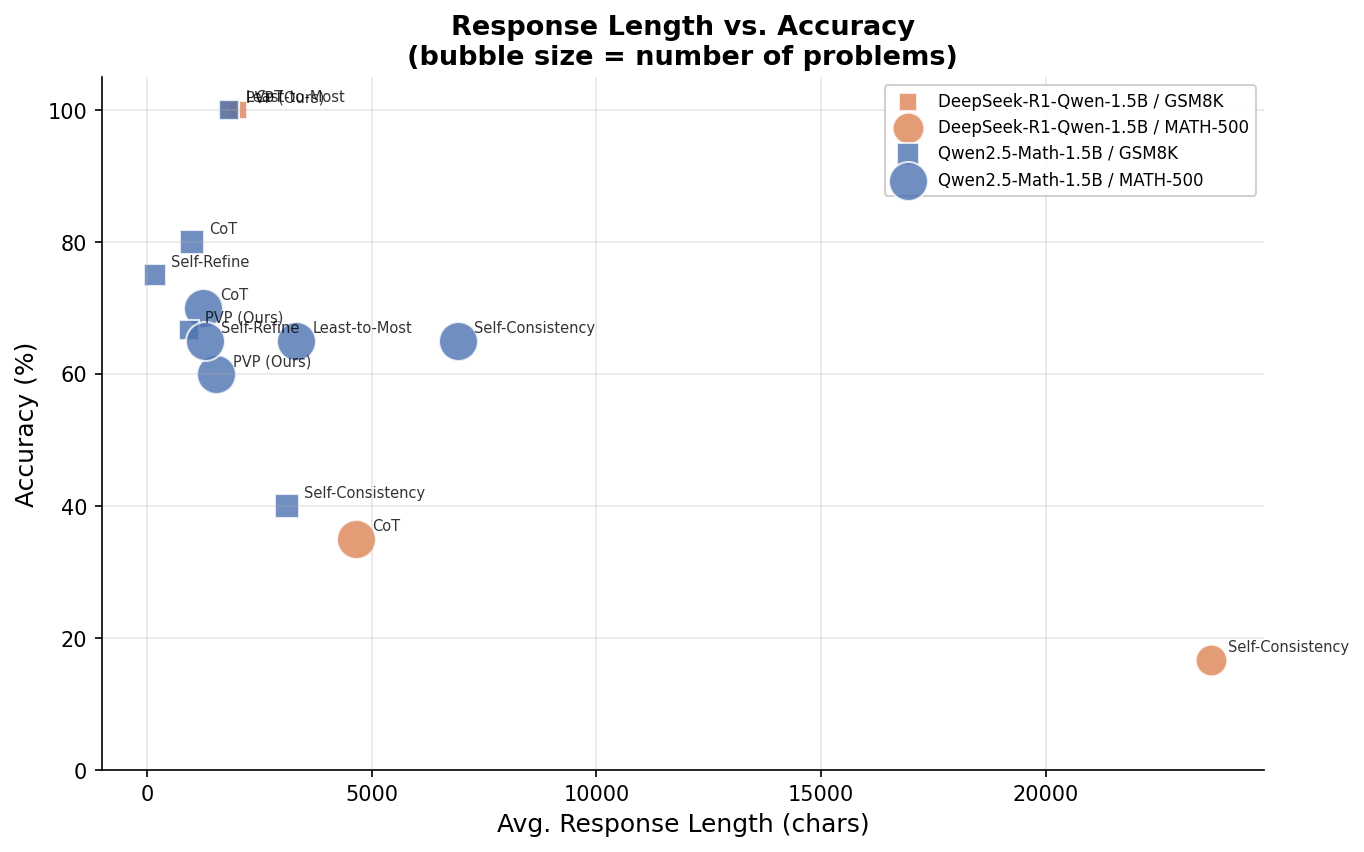
\includegraphics[width=3in]{../results/figures/fig6_length_vs_accuracy.png}
  \caption{Scatter plot of response length vs accuracy.}
  \label{fig:length}
\end{figure}

%==============================================================================
\section{Discussion}
%==============================================================================

\subsection{Finding 1: Model Choice Matters More Than Prompt Engineering}

Qwen2.5-Math-1.5B (65.8\%) dominates DeepSeek-R1-Qwen-1.5B (36.4\%) across all prompting strategies. A task-specific model with simple CoT (70.0\% on MATH-500) outperforms a general model with any advanced method. This suggests that for mathematical reasoning, domain-specific fine-tuning provides a stronger foundation than sophisticated prompting alone.

\subsection{Finding 2: Problem Decomposition Is Most Effective}

Least-to-Most achieves the highest accuracy (69.6\%) by decomposing complex problems into manageable sub-problems. This structured decomposition is particularly beneficial for small 1.5B models, as it reduces the effective reasoning chain length and allows the model to focus on simpler intermediate steps.

\subsection{Finding 3: Self-Consistency Struggles with Small Models}

Self-Consistency (44.4\%) underperforms the CoT baseline (57.5\%), contrary to results reported for larger models. With only 1.5B parameters, the models lack sufficient reasoning diversity---the 5 samples tend to either all succeed or all fail on the same problems, making majority voting ineffective. This finding suggests that Self-Consistency requires a minimum model scale threshold to be beneficial.

\subsection{Finding 4: Verification-Based Methods Show Promise}

Both Self-Refine (66.7\%) and PVP (64.0\%) outperform the CoT baseline, confirming that self-verification improves reasoning quality. PVP is particularly notable for achieving competitive accuracy with single-pass inference latency (${\sim}$25s vs Self-Refine's ${\sim}$90s), offering the best accuracy-efficiency trade-off among all methods tested.

\subsection{Finding 5: PVP Offers Best Efficiency Trade-off}

PVP provides competitive accuracy (${\sim}$64\%) with CoT-level latency (${\sim}$25s per problem). Compared to Self-Consistency (5$\times$ cost, lower accuracy) and Self-Refine (3$\times$ cost, slightly higher accuracy), PVP represents the most practical verification-based prompting strategy for resource-constrained settings.

%==============================================================================
\section{Limitations and Future Work}
%==============================================================================

\begin{enumerate}
    \item \textbf{Sample size}: Due to CPU inference constraints, most experiments used 20 samples per combination. Larger-scale experiments would yield more statistically robust conclusions.
    \item \textbf{Model scale}: Results are limited to 1.5B-parameter models. Advanced prompting strategies may be more effective with larger models (7B, 70B) where reasoning diversity is greater.
    \item \textbf{No AIME 2024 results}: The hardest benchmark dataset was not included in the final runs due to time constraints.
    \item \textbf{API models not fully evaluated}: GPT-4o-mini and DeepSeek Chat comparisons would provide cross-scale insights.
    \item \textbf{PVP design space}: The current PVP template uses a fixed verification structure. Adaptive verification (varying verification depth based on problem complexity) is a promising future direction.
\end{enumerate}

%==============================================================================
\section{Conclusion}
%==============================================================================

We presented a systematic evaluation of five prompting strategies for mathematical reasoning in LLMs, introducing Progressive Verification Prompting (PVP) as a novel approach. Our key findings demonstrate that: (1) task-specific models dramatically outperform general-purpose models regardless of prompting strategy; (2) problem decomposition (Least-to-Most) is the most effective strategy for small models; (3) Self-Consistency is counterproductive for small models; and (4) PVP offers a practical, efficient improvement over the CoT baseline by integrating step-wise verification directly into the reasoning process. Our open-source experimental framework supports reproducible evaluation with checkpoint/resume capabilities.

%==============================================================================
\section*{References}
%==============================================================================

\begin{thebibliography}{9}

\bibitem{wei2022}
J.~Wei, X.~Wang, D.~Schuurmans, et al.,
``Chain-of-thought prompting elicits reasoning in large language models,''
\textit{Advances in Neural Information Processing Systems (NeurIPS)}, 2022.

\bibitem{wang2022}
X.~Wang, J.~Wei, D.~Schuurmans, et al.,
``Self-consistency improves chain of thought reasoning in language models,''
\textit{Advances in Neural Information Processing Systems (NeurIPS)}, 2022.

\bibitem{madaan2024}
A.~Madaan, N.~Tandon, P.~Gupta, et al.,
``Self-refine: Iterative refinement with self-feedback,''
\textit{Advances in Neural Information Processing Systems (NeurIPS)}, 2024.

\bibitem{zhou2023}
D.~Zhou, N.~Sch\"{a}rli, L.~Hou, et al.,
``Least-to-Most Prompting Enables Complex Reasoning in Large Language Models,''
\textit{Advances in Neural Information Processing Systems (NeurIPS)}, 2023.

\bibitem{cobbe2021}
K.~Cobbe, V.~Kosaraju, M.~Bavarian, et al.,
``Training verifiers to solve math word problems,''
\textit{arXiv preprint arXiv:2110.14168}, 2021.

\bibitem{hendrycks2021}
D.~Hendrycks, C.~Burns, S.~Kadavath, et al.,
``Measuring Mathematical Problem Solving With the MATH Dataset,''
\textit{Advances in Neural Information Processing Systems (NeurIPS)}, 2021.

\bibitem{zhang2023}
Z.~Zhang, A.~Zhang, M.~Li, A.~Smola,
``Automatic Chain of Thought Prompting in Large Language Models,''
\textit{arXiv preprint arXiv:2210.03493}, 2022.

\bibitem{weng2023}
Y.~Weng, M.~Zhu, F.~Xia, et al.,
``Large Language Models are Better Reasoners with Self-Verification,''
\textit{arXiv preprint arXiv:2212.09561}, 2023.

\end{thebibliography}

%==============================================================================
\appendices
%==============================================================================

\section{PVP Prompt Template}
\label{sec:pvp_prompt}

\begin{lstlisting}
Solve the following math problem. Follow these instructions carefully:

1. Break the problem into clear reasoning steps.
2. After EACH step, pause and verify:
   - Is this step logically correct?
   - Does it follow from the previous step?
   - Are there any arithmetic errors?
   If you find an error, correct it immediately before proceeding.
3. After all steps, perform a final review to verify the overall solution
   is consistent.
4. Put your final answer in \boxed{}.

Problem: {problem}

Begin solving with progressive verification:
\end{lstlisting}

\section{All Prompt Templates}
\label{sec:all_prompts}

\subsection{CoT Template}

\begin{lstlisting}
Solve the following math problem step by step. Show your reasoning clearly
and put your final answer in \boxed{}.

Problem: {problem}

Please reason step by step:
\end{lstlisting}

\subsection{Self-Consistency Template}
Same as CoT (sampling is controlled at inference level with temperature $> 0$).

\subsection{Self-Refine Templates}
\textbf{Solve Phase}: Same as CoT.

\textbf{Critique Phase}:
\begin{lstlisting}
Review the following solution to a math problem. Identify any errors in
reasoning, calculation mistakes, or logical flaws. Be specific about
what is wrong and why.

Problem: {problem}
Solution to review: {solution}

Please provide your critique:
\end{lstlisting}

\textbf{Refine Phase}:
\begin{lstlisting}
Based on the critique below, improve the solution to the following math
problem. Fix any identified errors and provide the corrected solution.
Put your final answer in \boxed{}.

Problem: {problem}
Original solution: {solution}
Critique: {critique}

Please provide the improved solution:
\end{lstlisting}

\subsection{Least-to-Most Templates}
\textbf{Decompose Phase}:
\begin{lstlisting}
Break down the following math problem into simpler sub-questions. List them
in order from simplest to most complex. Each sub-question should build on
the previous ones.

Problem: {problem}

List the sub-questions:
\end{lstlisting}

\textbf{Solve Phase}:
\begin{lstlisting}
Here is a math problem and its decomposition into sub-questions:
Problem: {problem}
Sub-questions: {sub_questions}

Solve each sub-question in order. Use the answer from each sub-question
to help solve the next one. Put your final answer in \boxed{}.

Please solve step by step:
\end{lstlisting}

\section{System Architecture}
\label{sec:architecture}

The system consists of three layers:
\begin{enumerate}
    \item \textbf{Presentation Layer}: Streamlit Web Demo with interactive solver, dashboard (charts), and comparison analysis (model $\times$ method).
    \item \textbf{Experiment Runner}: Orchestrates experiments with checkpoint/resume support, configuration management, and JSON-based result storage.
    \item \textbf{Core Pipeline}: Data loader $\rightarrow$ Prompt engine $\rightarrow$ Model router $\rightarrow$ Evaluation (accuracy, metrics).
\end{enumerate}

\section{Visualization Charts}
\label{sec:charts}

The following 7 charts are generated from experimental data:
\begin{enumerate}
    \item \textbf{fig1\_accuracy\_by\_model.png} --- Bar chart comparing Qwen2.5-Math (65.8\%) vs DeepSeek-R1 (36.4\%).
    \item \textbf{fig2\_accuracy\_by\_method.png} --- Ranked bar chart of 5 methods (Least-to-Most $>$ Self-Refine $>$ PVP $>$ CoT $>$ SC).
    \item \textbf{fig3\_accuracy\_by\_dataset.png} --- GSM8K (75.0\%) vs MATH-500 (55.0\%).
    \item \textbf{fig4\_model\_x\_method.png} --- Grouped bar chart showing all model $\times$ method combinations.
    \item \textbf{fig5\_heatmap\_model\_method.png} --- Heatmap of accuracy across model $\times$ method matrix.
    \item \textbf{fig6\_length\_vs\_accuracy.png} --- Scatter plot of response length vs accuracy.
    \item \textbf{fig7\_latency\_by\_method.png} --- Bar chart of inference latency per method.
\end{enumerate}

\end{document}
